\begin{frame}\frametitle{Parton distribution functions}
\centering\small

  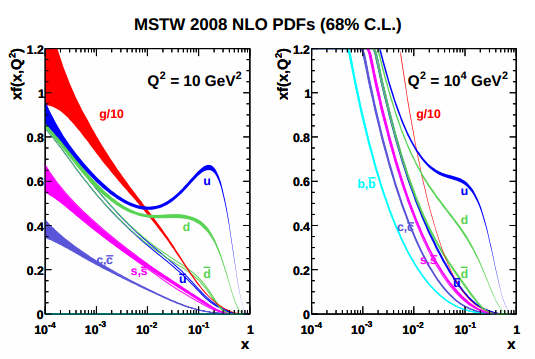
\includegraphics[width=0.6\textwidth]{../montecarlo/figures/pdfs2.png}

\myskip
standard PDFs $f_{a,b}(x_{a,b},\mu_{F})$ 
for partons $a,b = \{g,u,\bar{u},d,...\}$ 
 carrying fractions $x_a,x_b$ of the proton longitudinal momenta
$p_1, p_2$
\end{frame}



\begin{frame}\frametitle{Factorization theorem}
\centering\myskip

In any {\cccolor hard and inclusive} process ${\rm pp}\to{\rm X}$\\
can separate the {\cccolor soft} and {\cccolor hard} components:
$$
  \sigma_{{\rm pp}\to{\rm X}}
  = \sum_{a,b}
  \int_{0}^{1}{\rm d}x_a{\rm d}x_b
  ~ f_a(x_a,\mu_{F}) f_b(x_b,\mu_{F})
  \hat{\sigma}_{{\rm ab}\to{\rm X}}(x_ap_1, x_bp_2,\mu_R^2,\mu_{F}^2)
$$

short distance partonic cross section computable in fixed-order pQCD:
$$\hat{\sigma}_{{\rm ab}}=\sum_{i=0}^{n} \alphas^i \hat{\sigma}_i(x_ap_1, x_bp_2,\mu_R^2,\mu_{F}^2)=\hat{\sigma}_0+\alphas \hat{\sigma}_1+\dots$$

\begin{itemize}
\item $\mu_{F}$ = {\it factorization scale} 
\item arbitrary choice of the scale at which soft- and hard-interaction separate, in general $\mu_{R}$ (\alphas\ renormalization scale)
\end{itemize}

\end{frame}

